\section{Invariants}
\label{sec:invariants}

The caches are assumed to be organized in the form of a tree
(Figure~\ref{fig:hierarchy}). The leaves of this tree represent the L1 caches,
with each L1 cache connected to exactly one core. The root of the tree is a
single Last-level cache (LLC), connected to the main memory. A (cache) node can
communicate only with its parents or with its children via a request or
response message whose format is in Figure~\ref{message}.

\begin{figure}
\begin{tabularx}{\linewidth}{|X|}
\hline
\multicolumn{1}{|c|}{Blocking restrictions}\\
\hline
\begin{enumerate}
\item A request from a child should not block the handling of a request from
the parent, even for a different address.
\item Requests for an address $a$ should not block the handling of responses
for address $a$, even from a different source.
\end{enumerate}\\
\hline
\multicolumn{1}{|c|}{Ordering requirements}\\
\hline
\begin{enumerate}
\item A response for an address $a$ from a child $c$ should not be received
before a response from the same $c$ and the same $a$ sent earlier has been
received.
\item The handling of a request for an address $a$ from a source $n$ should not
be started before a response from the same $n$ for the same $a$ sent earlier
has been received.
\end{enumerate}\\
\hline
\end{tabularx}
\caption{Blocking restrictions and order of receiving messages}
\label{receiveOrder}
\end{figure}

The restrictions of which messages can not block each other, and the order in
which messages should be received and handled is given in
Figure~\ref{receiveOrder}.

One way to implement the ordering restrictions is to have a network which
guarantees FIFO ordering between any two nodes. Having one virtual channel for
the messages from the parent and another for the messages from the children
enforces the blocking restriction between requests from the parent and the
children. Among messages from the parent (or the children), having two virtual
channels, one for requests and one for responses, with responses having higher
priority than requests enforces the blocking restrictions and the ordering
requirements between requests and responses. Such an organization is shown in
Figure~\ref{fig:network}.

Note that the organization in Figure~\ref{fig:network} requires finishing
processing of a request from a child before starting the processing of the
request from another child, or for a different address. It makes the node
behave more like a blocking cache, whose performance may be low. The
restrictions given in Figure~\ref{receiveOrder} however do not impose this
organization. One can process requests to different addresses in any order,
using MSHRs.

The ordering requirements of Figure~\ref{receiveOrder} can be enforced using
prioritized virtual channels which guarantee FIFO ordering between messages
sent from the same source to the same destination (as discussed above).
However, as we show later, the ordering requirements can be enforced even when
the underlying network does not guarantee FIFO ordering between two nodes.

The values of the coherence state (and hence the directory state) belong to a
totally ordered set, \ie a set in which a \emph{less than} ($<$) relation is
defined between any two set elements and this relation is transitive. If an
address is not present, then the coherence state corresponding to that address
is the lowest value in the set (which we denote by \Inv). For instance, in an
MSI protocol, the values of the coherence state are from the set $\{M, S, I\}$
where $I < S$, $S < M$ and $I < M$; if an address is not present, the state
corresponding to that address is $I$. Our abstract protocol does not assign any
semantics or meaning to the values of the coherence states. In a concrete cache
coherence protocol, the values of the states are associated with permissions
for reading and writing, and the state with fewer permissions is less than the
state with more permissions.

\begin{figure}\centering
\begin{tabularx}{\linewidth}{|l|X|}
\hline
$state[a]$ & Coherence state for address $a$\\
\hline
$dir[a][c]$ & Directory's version of the coherence state for address $a$ in child
$c$\\
\hline
\end{tabularx}
\caption{Information stored for each cache line}
\label{table:storage}
\end{figure}

\begin{figure}\centering
\begin{tabularx}{\linewidth}{|l|X|}
\hline
$isPresent(a)$ & Is line for address $a$ present in this node?\\
\hline
$isWait(n, a)$ & Is there a pending response from node $n$ (either parent $P$
or a child) for address $a$?\\
\hline
$isEvicting(a)$ & Is address $a$ currently being evicted?\\
\hline
%$isEnterPending(a)$ & Is there any (child) request for address $a$ waiting to get
%a cache line entry in the cache?\\
%\hline
$isHandling(n, a)$ & Is there any request for address $a$ from node $n$ (either
parent $P$ or a child) that is being handled?\\
\hline
%$replacingAddr(a)$ & The address that is going to replace the line
%corresponding to address $a$\\
%\hline
%$cWaitState(c, a)$ & The state to which the node has requested its child $c$ to
%downgrade to and hence waiting for a response\\
%\hline
\end{tabularx}
\caption{Information that can be computed for each address (typically from the
MSHR)}
\label{table:functions}
\end{figure}

%\begin{figure}
%\begin{tabularx}{\linewidth}{|l|l|X|}
%\hline
%\multicolumn{3}{|c|}{\Req{n}{a}{x}}\\
%\hline
%\multirow{4}{*}{$n = P$} & Incoming & Request from parent for changing my
%                                      $state[a]$ to $x$\\
%\cline{2-3}
%                         & Outgoing & Request to parent for permission to change
%                                      my $state[a]$ to $x$\\
%\hline
%\multirow{4}{*}{$n \neq P$} & Incoming & Request from child $n$ for permission
%                                         to change $n$'s $state[a]$ to $x$\\
%\cline{2-3}
%                            & Outgoing & Request to child $n$ to change $n$'s
%                                         $state[a]$ to $x$\\
%\hline
%\multicolumn{3}{|c|}{\Resp{n}{a}{x}}\\
%\hline
%\multirow{4}{*}{$n = P$} & Incoming & Response from parent granting permission
%                                      to change my $state[a]$ to $x$\\
%\cline{2-3}
%                         & Outgoing & Response to parent indicating that my
%                                      $state[a]$ has changed to $x$\\
%\hline
%\multirow{4}{*}{$n \neq P$} & Incoming & Response from child indicating that
%                                         $n$'s $state[a]$ has changed to $x$\\
%\cline{2-3}
%                            & Outgoing & Response to child $n$ granting permission
%                                         to change $n$'s $state[a]$ to $x$\\
%\hline
%\end{tabularx}
%\caption{Incoming and outgoing messages}
%\label{table:messages}
%\end{figure}

\begin{figure}
\begin{tabularx}{\linewidth}{|X|}
\hline
\begin{enumerate}
\item[] A response for address $a$ can be sent only if the line for $a$ is present in
the current node, \ie $isPresent(a)$
\end{enumerate}\\
\hline
\multicolumn{1}{|c|}{Response to child $c$ for address $a$, \Resp{c}}\\
\hline
\begin{enumerate}
\item A response to child $c$ for address $a$ can be sent only if a
request from child $c$ for $a$ is being handled, \ie $isHandling(c, a)$
\item Response \Resp{c}{a}{x} can be sent only if $x > dir[a][c]$
% $\forall c', c' \neq c \rightarrow isCompatible(x, dir[a][c'])$ and  $x \le state[a]$
\end{enumerate}\\
\hline
\multicolumn{1}{|c|}{Response to parent $P$ for address $a$}\\
\hline
\begin{enumerate}
\item If there is a pending response from the parent for address $a$, \ie $
isWait(P, a)$, a response to the parent for $a$ can be sent only if a request
from the parent for $a$ is being handled, \ie $isHandling(P, a)$
\item If there is no pending response from the parent for address $a$, \ie
$\neg isWait(P, a)$, a response to the parent for $a$ can be sent any time
\item Response \Resp{P}{a}{x} can be sent only if $x < state[a]$
% and $\forall c, x \ge dir[a][c]$
\end{enumerate}\\
\hline
\end{tabularx}
\caption{Sending a response: Preconditions}
\label{sendRespPre}
\end{figure}

\begin{figure}
\begin{tabularx}{\linewidth}{|X|}
\hline
\begin{enumerate}
\item[] A response for address $a$ can be sent only if the line for $a$ is
present in the current node, \ie $isPresent(a)$
\end{enumerate}\\
\hline
\multicolumn{1}{|c|}{Response to child $c$ for address $a$}\\
\hline
\begin{enumerate}
\item[] On sending \Resp{c}{a}{x}, $dir[a][c]$ changes to $x$
\end{enumerate}\\
\hline
\multicolumn{1}{|c|}{Response to parent $P$ for address $a$}\\
\hline
\begin{enumerate}
\item[] On sending \Resp{P}{a}{x}, $state[a]$ changes to $x$
\end{enumerate}\\
\hline
\end{tabularx}
\caption{Sending a response: Side effects}
\label{sendRespEff}
\end{figure}

\begin{figure}
\begin{tabularx}{\linewidth}{|X|}
\hline
\multicolumn{1}{|c|}{On receiving a response \Resp{c}{a}{x}}\\
\hline
\begin{enumerate}
\item $dir[a][c]$ changes to $x$
\item Response \Resp{c}{a}{x} is removed
\item $isWait(c, a)$ is set \False
\end{enumerate}\\
\hline
\multicolumn{1}{|c|}{On receiving a response \Resp{P}{a}{x}}\\
\hline
\begin{enumerate}
\item $state[a]$ changes to $x$
\item Response \Resp{P}{a}{x} is removed
\item $isWait(P, a)$ is set \False
\end{enumerate}\\
\hline
\end{tabularx}
\caption{Receiving a response: Effects}
\label{recvResp}
\end{figure}

\floatstyle{boxed}
\restylefloat{figure}

\begin{figure}
\begin{enumerate}
\item $state[a]$ can change only on sending or receiving a response from the
parent
\item $dir[a][c]$ can change only on sending or receiving a response from child
$c$
\end{enumerate}
\caption{State and directory changes: Preconditions}
\label{stateChange}
\end{figure}

\floatstyle{plain}
\restylefloat{figure}

\begin{figure}
\begin{tabularx}{\linewidth}{|X|}
\hline
\multicolumn{1}{|c|}{Request to child $c$ for address $a$}\\
\hline
\begin{enumerate}
\item A request can be sent to child $c$ for address $a$ only if there is no
pending response from child $c$ for $a$, \ie $\neg isWait(c, a)$
\item Request \Req{c}{a}{x} can be sent only if $x < dir[a][c]$
\end{enumerate}\\
\hline
\multicolumn{1}{|c|}{Request to parent $P$ for address $a$}\\
\hline
\begin{enumerate}
\item A request can be sent to the parent for address $a$ only if
  \begin{enumerate}
  \item there is no pending response from the parent for address $a$, \ie
  $\neg isWait(P, a)$, and
  \item line in address $a$ is not being evicted, \ie $isEvicting(a)$
  \end{enumerate}
\item Request \Req{P}{a}{x} can be sent only if $x > state[a]$
\end{enumerate}\\
\hline
\end{tabularx}
\caption{Sending a request: Preconditions}
\label{sendReq}
\end{figure}

\begin{figure}
\begin{tabularx}{\linewidth}{|X|}
\hline
\multicolumn{1}{|X|}{\centering Request \Req{c}{a}{x} from child $c$ is being handled, \ie
$isHandling(c, a)$}\\
\hline
\begin{enumerate}
\item[] If $x \le state[a] \wedge \forall c'\neq c, isCompatible(x, dir[a][c])$,
 then a response \Resp{c}{a}{x} is sent to $c$ if $x > dir[a][c]$
%\item If $x = \Inv$ then data for address $a$ is transferred to $c$
\end{enumerate}\\
\hline
\multicolumn{1}{|c|}{Address $a$ is marked as being evicted, \ie $isEviting(a)$}\\
\hline
\begin{enumerate}
\item[] If $\forall c, dir[a][c] \le \Inv$, a response \Resp{P}{a}{\Inv} is sent
to the parent if $\Inv < state[a]$
%\item If $state[a] \in \Dirty$ then data for address $a$ is transferred to $c$
\end{enumerate}\\
\hline
\multicolumn{1}{|X|}{\centering Request \Req{P}{a}{x} from parent $P$ is being
handled, \ie $isHandling(P, a)$}\\
\hline
\begin{enumerate}
\item[] If $\forall c, dir[a][c] \le x$, a response \Resp{P}{a}{x} is sent to the
parent if $x < state[a]$
%\item If $state[a] \in \Dirty$ then data for address $a$ is transferred to the parent
\end{enumerate}\\
\hline
\end{tabularx}
\caption{Forced responses: Effects}
\label{respForReq}
\end{figure}

\begin{figure}
\begin{tabularx}{\linewidth}{|X|}
\hline
\multicolumn{1}{|c|}{Request \Req{c}{a}{x} from child $c$ is received}\\
\hline
\begin{enumerate}
\item If address $a$ is present in the node, \ie $isPresent(a)$, handling of
request \Req{c}{a}{x} can be started, \ie $isHandling(c, a)$ can be set \True
only if
  \begin{enumerate}
  \item no request \Req{n}{a}{x} from any node $n$ for address $a$ is being
  handled, \ie $\forall n, \neg isHandling(n, a)$
  \item address $a$ is not currently being evicted, \ie $\neg isEvicting(a)$
  \end{enumerate}
\item If $a$ is not present in the node, \ie $\neg isPresent(a)$, handling of
request \Req{c}{a}{x} can be started \ie $isHandling(c, a)$ can be set \True
only if there is a line with address $a'$ such that
  \begin{enumerate}
  \item no request \Req{n}{a'}{x} from any node $n$ for address $a'$ is being
  handled, \ie $\neg isHandling(n, a')$
  \item address $a'$ is not currently being evicted, \ie $\neg isEvicting(a')$
  \end{enumerate}
\end{enumerate}\\
\hline
\multicolumn{1}{|c|}{Request \Req{P}{a}{x} from parent $P$ is received}\\
\hline
\begin{enumerate}
\item[] Handling of request \Req{P}{a}{x} can be started \ie $isHandling(P, a)$
can be set \True, only if there are no pending responses from any child for
address $a$, \ie $\forall c \in Children, \neg isWait(c, a)$
\end{enumerate}\\
\hline
\end{tabularx}
\caption{Start handling a request: Preconditions}
\label{respForReqPre}
\end{figure}

\begin{figure}
\begin{tabularx}{\linewidth}{|X|}
\hline
\multicolumn{1}{|c|}{Request \Req{c}{a}{x} from child $c$ is received}\\
\hline
\begin{enumerate}
\item Handling of the request \Req{c}{a}{x} has started, \ie $isHandling(c, a)$
is set \True
\item If $a$ is not present in the node, \ie $\neg isPresent(a)$, a line with
address $a'$ is found such that
  \begin{enumerate}
  \item no request \Req{n}{a'}{x} from any node $n$ for address $a'$ is being
  handled, \ie $\forall n, \neg isHandling(n, a')$
  \item address $a'$ is not currently being evicted, \ie $\neg isEvicting(a')$
  \end{enumerate}
$a'$ is marked as being evicted, \ie $isEvicting(a')$ is set \True
\end{enumerate}\\
\hline
\multicolumn{1}{|c|}{Request \Req{P}{a}{x} from parent $P$ is received}\\
\hline
\begin{enumerate}
\item[] Handling of the request \Req{P}{a}{x} is started, \ie $isHandling(P, a)$ is set \True
\end{enumerate}\\
\hline
\end{tabularx}
\caption{Start handling a request: Effects}
\label{respForReqEff}
\end{figure}

\begin{figure}
\begin{tabularx}{\linewidth}{|X|}
\hline
\multicolumn{1}{|c|}{Request \Req{c}{a}{x} from child $c$ is being handled}\\
\hline
\begin{enumerate}
\item If $x \le dir[a][c]$, the request is removed
\item $isHandling(c, a)$ is set \False
\end{enumerate}\\
\hline
\multicolumn{1}{|c|}{Request \Req{P}{a}{x} from parent $P$ is being
handled}\\
\hline
\begin{enumerate}
\item If $x \ge state[a]$, the request is removed
\item $isHandling(P, a)$ is set \False
\end{enumerate}\\
\hline
\end{tabularx}
\caption{Finish handling a request: Effects}
\label{finishHandle}
\end{figure}

\begin{figure}
\begin{tabularx}{\linewidth}{|X|}
\hline
Request \Req{c}{a}{x} from child $c$ is being handled, and address $a'$ is
replaced by $a$\\
\hline
\begin{enumerate}
\item If $state[a'] <= \Inv$, address $a'$ for the line is replaced by $a$, \ie
$isPresent(a')$ is set \False and $isPresent(a)$ is set \True
\item $state[a']$ is set \Inv and $\forall c, dir(c, a)$ is set \Inv
\item $a'$ is no longer being evicted, \ie set $isEvicted(a')$ to \False
\end{enumerate}\\
\hline
\end{tabularx}
\caption{Finish replacing line: Effects}
\end{figure}

\begin{figure}
\centering
\begin{subfigure}{\linewidth}
\centering
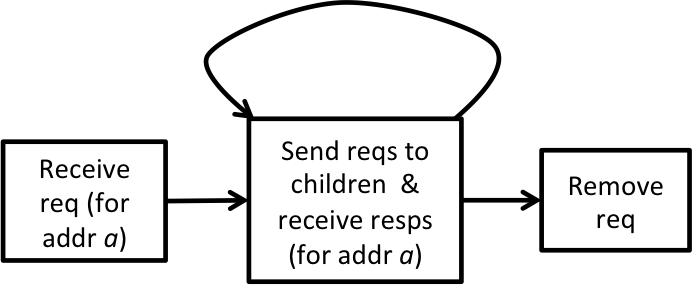
\includegraphics[scale=0.5]{reqFromP}
\caption{Stages in handling a request from parent}
\label{fig:reqFromP}
\end{subfigure}

\begin{subfigure}{\linewidth}
\centering
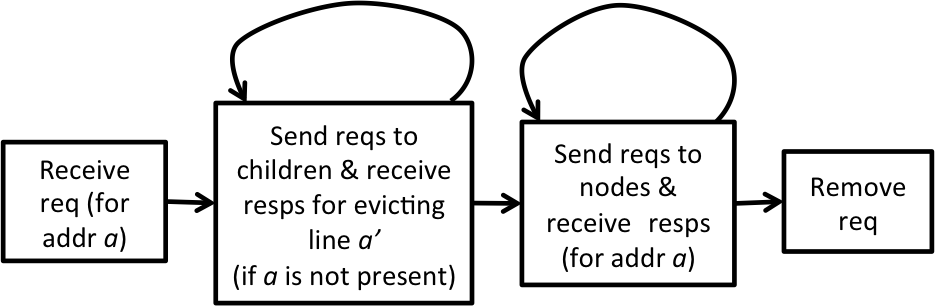
\includegraphics[scale=0.5]{reqFromC}
\caption{Stages in handling a request from a child}
\label{fig:reqFromC}
\end{subfigure}
\end{figure}

\begin{figure}
\begin{tabularx}{\linewidth}{|X|}
\hline
\begin{enumerate}
\item If a request that is being handled requires $state[a]$ to be $x$ while
currently $state[a] < x$ and there is no pending response from the parent for
$a$, \ie $\neg isWait(P, a)$, a request \Req{P}{a}{x} is sent to the parent and
$isWait(P, a)$ is set \True
\item If a request that is being handled requires $dir[a][c]$ for some $c$ to
be $x$ while currently $dir[a][c] > x$ and there is no pending response from
child $c$, \ie $\neg isWait(c, a)$, a request \Req{c}{a}{x} is sent to $c$ and
$isWait(c, a)$ is set
\True
\end{enumerate}\\
\hline
\end{tabularx}
\caption{Handling of an incoming request: Effects}
\label{handling}
\end{figure}

\begin{figure}
\begin{tabularx}{\linewidth}{|X|}
\hline
\begin{enumerate}
\item The effects during sending a response or sending a request is atomic,
\ie if there is no space available in the sending buffer, then the action is
aborted without causing any effect and retried later
\item The effect of abort can be achieved by checking if the required resources
are available before starting the action 
\end{enumerate}\\
\hline
\end{tabularx}
\caption{Atomicity requirements}
\label{atomicity}
\end{figure}
